\documentclass[12pt]{report}

% ---------- Packages (safe defaults) ----------
\usepackage[a4paper,margin=1in]{geometry}
\usepackage{graphicx}
\usepackage{setspace}
\usepackage{float}
\usepackage{booktabs}
\usepackage{hyperref}
% --- Code snippets ---
\usepackage{xcolor}
\usepackage{listings}

\lstdefinestyle{code}{
  basicstyle=\ttfamily\small,
  numbers=left,
  numberstyle=\tiny,
  stepnumber=1,
  numbersep=8pt,
  frame=single,
  framerule=0.4pt,
  breaklines=true,
  breakatwhitespace=true,
  tabsize=2,
  showstringspaces=false,
  captionpos=b,
  keywordstyle=\color{blue},
  commentstyle=\color{gray},
  stringstyle=\color{teal},
}

% --- References ---
\usepackage[backend=biber,style=authoryear]{biblatex}
\addbibresource{refs.bib}

% Default style
\lstset{style=code}

\title{Deep Learning for Breast Cancer Detection in Mammography}
\author{Tom Parrott}
\date{\today}

\begin{document}

% ---------- Title page ----------
\begin{titlepage}
    \centering
    \vspace*{3cm}

    {\LARGE \textbf{Deep Learning for Breast Cancer Detection in Mammography}\par}
    \vspace{1.5cm}

    {\Large Tom Parrott\par}
    \vspace{0.5cm}

    {\large CM3070 Final Project\par}
    \vspace{0.5cm}

    {\large University of London\par}
    \vspace{1.5cm}

    {\large February 2026\par}

    \vfill
\end{titlepage}

% ---------- Abstract (placeholder) ----------
\begin{abstract}
\noindent
\textbf{Placeholder:} This project investigates whether deep learning can improve breast cancer detection from mammography images. The final version of this abstract will summarise the dataset used, model approach (baseline vs experiments), evaluation design (patient-level splitting and clinically relevant metrics), key results, and main conclusions.
\end{abstract}

\clearpage

% ---------- Table of contents + lists ----------
\tableofcontents
\clearpage

\listoffigures
\clearpage

\listoftables
\clearpage

\section{Introduction}

For this project, I have selected the Machine Learning and Neural Network template, Deep Learning
Breast Cancer Detection. The central question this project seeks to address is: Can deep learning improve
the accuracy of breast cancer detection from mammography images? In exploring this question, the
project focuses on the application of transfer learning to medical imaging data, with the aim of improving
detection performance while maintaining clinical relevance.(Litjens et al., 2017; Ragab et al., 2022).

There were two primary reasons for choosing this topic, one academic and one personal. Academically,
the Machine Learning and Neural Networks module was the most engaging module I undertook at level 6
so far. This project provides an opportunity to deepen my understanding of deep learning techniques and
to apply them in a realistic, data driven context. Looking ahead, I intend to pursue either postgraduate
study or professional work involving machine learning, and this project allows me to develop skills that
are directly relevant to that goal. On a personal level, breast cancer is a disease with significant real-world
impact. Having lost my mother to cancer that metastasised following delayed treatment, this project holds
personal importance and reinforces my motivation to explore how machine learning might contribute to
earlier and more reliable diagnoses in the future.

Breast cancer is the most common cancer in the UK, accounting for approximately 15\% of all new cancer
cases and around 30\% of cancers diagnosed in women. Each year, over 56,000 new cases are diagnosed
in the UK, and approximately one in seven women will develop breast cancer during their lifetime
(Cancer Research UK, 2023). Globally, breast cancer remains a major public health concern, with 2.3
million diagnoses and 670,000 deaths reported worldwide in 2022 according to the World Health
Organisation (World Health Organization, 2022). These statistics highlight the scale of the problem and
provide strong justification for continued research into improving screening and diagnostic processes.

Cancer is typically classified into four stages, which describe how far the disease has progressed at the
time of diagnosis (National Cancer Institute, 2023). Early-stage cancers are confined to their original
tissue, while later stages indicate a spread to nearby lymph nodes or further away organs. This spread,
known as metastasing, occurs when cancer cells break away from the primary tumour and travel through
the bloodstream or lymphatic system (American Cancer Society, 2022). Metastasised cancer is
significantly more difficult to treat and is associated with poorer outcomes and a higher mortality rate. As
a result, early detection plays a crucial role in improving survival rates. When breast cancer is diagnosed
at an early stage, treatment is more effective and the likelihood of long-term survival is substantially
higher (Cancer Research UK, 2023).

Breast cancer screening programmes aim to identify cancer before symptoms develop; however, the
current screening process has its limitations. In the UK and many other countries, there is a shortage of
specialist breast radiologists, leading to increased workloads and time pressure (NHS England, 2023).
Accuracy can vary depending on experience, clinician fatigue, and breast tissue density, which can
obscure tumours on standard mammograms (Elmore et al., 2015). These factors contribute to both false
positives, which can lead to unnecessary biopsies and anxiety, and false negatives, which delay diagnosis
and treatment (McKinney et al., 2020).

Machine learning, and deep learning in particular, offers the potential to address some of these challenges.
Convolutional neural networks have demonstrated strong performance in image-based classification tasks
by learning complex feature representations directly from raw pixel data (Esteva et al., 2017; Litjens et
al., 2017). In the context of mammography, deep learning models may be able to identify subtle patterns
that are difficult for the human eye to distinguish, particularly in dense breast tissue, which can be a real
issue for a lot of patients (Shen et al., 2017; McKinney et al., 2020). Rather than replacing clinicians, such
systems are increasingly viewed as decision support tools that can assist radiologists by highlighting
suspicious cases and reducing workload pressure (McKinney et al., 2020).

This project will aim to explore the use of deep learning techniques for breast cancer detection using
mammography images. In particular, it will look at whether CNNs, when trained on existing medical
imaging datasets, have the potential to identify patterns associated with breast cancer (Litjens et al.,
2017). The project aims to examine the feasibility of this approach within the context of current screening
practices.


\section{Literature Review}

Deep learning research advances have led to significant interest in applying convolutional neural networks (CNNs) to a wide range of computer vision problems, including breast cancer detection from mammography images (Litjens et al., 2017; Shen et al., 2017). CNN-based models learn hierarchical feature representations directly from pixel-level data, enabling the detection of subtle visual patterns that may be difficult to identify using traditional rule-based or handcrafted feature approaches. In contrast, earlier computer-aided detection (CAD) systems relied heavily on predefined features and heuristic rules, which limited their ability to generalise across diverse patient populations and imaging conditions, particularly in cases involving dense breast tissue (Elmore et al., 2015; Dromain et al., 2013).

As of 2025, CNNs appear to have become the dominant modelling approach in mammography research due to their ability to automatically extract discriminative spatial features from medical images. Numerous studies report strong performance when applying CNNs to classify mammograms as benign or malignant under controlled experimental conditions (Shen et al., 2017; McKinney et al., 2020; Ragab et al., 2022).

In the review published by Wang et al. (2024) they examined over 60 deep learning-based mammography studies and reported area under the curve (AUC) values ranging between 0.77 to 0.98. AUC measures how well a model can distinguish between classes by summarising its performance across all classification thresholds; a higher AUC indicates better overall discriminative ability. While these results demonstrate strong discriminative performance under controlled conditions, the review highlights substantial variation in evaluation methodology, including inconsistent use of metrics and frequent reliance on image level rather than patient level validation. This raises concerns regarding data leakage and inflated performance estimates, particularly in screening contexts where generalisation to unseen patients is critical. This data leakage can occur when information from outside the training data is unintentionally used to build a model, leading to unrealistically good performance and poor generalisation to new data.

The availability of publicly accessible datasets has played a crucial role in aiding deep learning research in mammography. The Digital Database for Screening Mammography (DDSM) has generally been one of the most widely used datasets; however, inconsistencies in annotation and metadata posed challenges for reproducibility (Heath et al., 2001; Lee et al., 2017).

To address these limitations, Lee et al. (2017) introduced the Curated Breast Imaging Subset of DDSM (CBIS-DDSM), which provides standardised labels, preprocessing pipelines, and patient identifiers. This dataset has since become a benchmark for CNN-based mammography studies and supports more rigorous experimental design, including patient level splitting strategies.

One issue highlighted within the literature review is data scarcity; there are too few high quality, labelled examples available to train a model effectively; CBIS-DDSM is still relatively small when compared to datasets typically used to train deep neural networks in other domain areas. This data scarcity presents challenges for training deep architectures from scratch, increasing the risk of overfitting.

To address this, numerous studies have adopted transfer learning approaches, leveraging pre-trained networks such as VGC, ResNet and EfficientNet.(Shen et al., 2017; Ragab et al., 2022; Huynh et al., 2016) Transfer learning models are pre-trained on large scale natural image datasets and are fine-tuned for domain specific tasks.

Ragab et al. (2022) reviewed the application of transfer learning in breast cancer detection and reported that fine-tuning pre-trained CNNs generally improves performance on small mammography datasets compared to training from scratch. This improvement is attributed to the reuse of low-level and mid-level feature representations learned from large datasets, which can accelerate convergence and reduce overfitting.

However, Ragab et al. (2022) also caution that transfer learning introduces potential risks related to domain mismatch, as natural images differ substantially from medical images in texture, scale, and semantic structure. Without careful fine-tuning and regularisation, transferred features may encode biases that reduce generalisability. These concerns highlight the need for careful architectural and training design when applying transfer learning in medical contexts.

In 2025, Kaddes et al. (2025), hybrid architectures have been explored that combine CNN features extraction with sequence-based models. Kaddes et al. (2025) proposed a CNN-LSTM hybrid model, where the CNN extracts spatial features from mammography images and the long short-term memory (LSTM) network models sequential dependencies within the extracted features; it reported an accuracy of 98.4\% on the CBIS-DDM dataset, demonstrating the potential of hybrid architectures to improve predictive performance. While these results illustrate the potential of advanced architectures, accuracy is seen as the primary metric and they do not evaluate performance at clinically relevant operating points, which would be something clinicians would need data on to ascertain if these models would be fit for purpose in real-world medical scenarios and be trusted by medical professionals that would seek to use them to aid in their work.

Across the reviewed literature, three modelling strategies appear most prominent: CNNs trained from scratch, transfer learning based CNNs and hybrid architectures (Wang et al., 2024; Ragab et al., 2022). Each approach prioritises different objectives and presents different trade-offs as a result.

CNNs trained from scratch offer greater domain specific feature learning and architectural transparency but are heavily constrained by data scarcity. Transfer learning improves data efficiency and performance on small datasets but introduces reliance on features learned from non-medical domains. Hybrid architectures prioritise raw performance by modelling higher order relationships but increase model complexity and reduce interpretability (Ragab et al., 2022; Wang et al., 2024).

No single approach consistently addresses all challenges associated with mammography screening. Instead, the various papers suggest that methodological rigor in validation and evaluation may be as important as architectural sophistication in achieving clinically meaningful results (Wang et al., 2024; McKinney et al., 2020).

Evaluation strategy is a critical factor in determining the real-world usefulness of deep learning models. Many mammography studies report accuracy or ROC-AUC as primary metrics; however, these measures may be misleading in highly imbalanced datasets, where cancer-positive cases are rare. When considering the number of patients that are screened for breast cancer in the UK alone per year, compared to the number of mammograms that test positive for cancer, the balance skews massively towards negative results. According to NHS Digital, around 2.2 million breast cancer screenings took place in 2022, of those, around 19,000 detected cancer in the patient; around 0.9\%, meaning around 99\% of all screenings return a negative screening result. From a human perspective, this is a good thing as nobody wants to be diagnosed with cancer, however, from a data science perspective, this creates a high data imbalance. 

In such scenarios, high accuracy can be achieved even when a model performs poorly on the minority class. Saito and Rehmsmeier (2015) demonstrated that precision–recall metrics and F1-score provide more informative evaluation in imbalanced classification tasks, as they explicitly capture the balance between false positives and false negatives.

From a clinical perspective, false negatives are particularly critical, as missed diagnoses may delay treatment and worsen patient outcomes. Screening programmes often operate at fixed specificity thresholds, making sensitivity at fixed specificity a more meaningful metric than aggregate AUC. Despite this, Wang et al. (2024) note that few studies report such clinically relevant measures, limiting the interpretability of reported performance.

Of the more recent papers (McKinney et al., 2020; Topol, 2019) emphasis has been increasing in deep learning systems to be designed as decision support tools rather than autonomous diagnostic ages, creating more of a human in the loop AI tool. Generally, clinicians require the highest level of reliability, so the ability for an expert to override autonomous decisions when there is a level of uncertainty is something that should be considered.

Human in the loop approaches, where models flag high risk or uncertain cases for further review would reduce the risk of becoming over reliant on algorithmic output and align with ethical and regulatory requirements (Topol, 2019; EU AI Act, 2023). However, it seems that a principle following a type of uncertainty estimation or a confidence calibration to involve a human seems relatively underexplored from the literature reviewed in this case study.

One of the main challenges highlighted in the literature, and one that would benefit from such a flagging system, is the variation in breast density, which significantly affects both human and algorithmic interpretation of images. Dense breast tissue appears radiopaque on mammograms, often obscuring lesions and reducing contrast between malignant and normal regions. Studies have shown (Boyd et al., 2007; Kerlikowske et al., 2010) that breast density is associated with increased rates of false negatives in traditional screening, highlighting an important limitation of both radiologist led and automated detection approaches.

Deep learning models can partially mitigate this challenge by learning more complex texture patterns beyond simple density intensity differences. However, Wang et al. (2024) note that many studies fail to stratify performance by breast density, making it difficult to assess whether reported improvements generalise across different patient subgroups. Without density aware evaluation, models may demonstrate strong average performance while still underperforming in clinically challenging cases. This omission represents a further gap in the literature, particularly given the clinical importance of dense breast tissue in screening populations, though gathering the data required for such a task presents an additional issue in itself.

Another significant challenge is generlisation beyond the training dataset, which is a challenge for machine learning in all medical settings, not just breast cancer screening. Many mammography studies evaluate models exclusively on internal test splits derived from the same dataset used for training. While such evaluations may indicate strong performance, they provide limited insight into how models will behave when exposed to data from different institutions, imaging devices, or patient demographics. Something that can be an issue as mentioned earlier with the imbalanced datasets in real world scenarios where the proportion of positive tests is under 1\% of the dataset.

Wang et al. (2024) highlight that only a small subset of reviewed studies perform external validation on independent datasets. This lack of external testing raises concerns regarding reliability and real-world applicability. Differences in image acquisition protocols, scanner manufacturers, and population characteristics can substantially affect model performance. For example, from what I was able to find, there were over 25 different manufacturers for mammography scanners, some of which use slightly different techniques. The Siemens Healthineers system generally uses direct conversion detectors, which give a sharp, high frequency noise profiles, whereas the GE HelathCare systems use indirect conversion detectors, which result in images with a smoother texture (Pisano et al., 2008; Vedantham et al., 2015). Consequently, models that perform well on curated benchmark datasets may experience performance degradation when deployed in clinical environments due to some of these hard-to-calculate variations.

Although full external validation may be beyond the scope of my project, being aware of these limitations will help in my evaluation of the success of the final output. 

In a healthcare setting, interpretability is generally recognised as a key requirement when deciding whether to adopt deep learning systems in healthcare, understanding how the decisions have been made is critical. A criticism sometimes directed towards CNNs is that they are ‘block box’ models (Rudin, 2019), producing predictions without explicit explanations of the underlying reasoning. From the point of view of a medical care provider, the lack of transparency can hinder trust and raise concerns.

Other studies (Selvaraju et al., 2017) attempt to address interpretability through techniques such as saliency maps or gradient based visualisations, which highlight image regions contributing most strongly to model predictions. However, Wang et al. (2024) caution that such visualisations are not always reliable indicators of true model reasoning and may provide misleading reassurance if interpreted uncritically.

The literature therefore suggests a trade-off between predictive performance and interpretability. More complex architectures, including hybrid models, may achieve higher accuracy but further obscure the decision-making process, a black box-like scenario. This trade-off reinforces the importance of positioning deep learning systems as decision support tools rather than autonomous diagnostic agents, particularly in high risk screening scenarios.

Beyond technical performance, ethical considerations play a crucial role in evaluating the suitability of AI systems for medical use. Breast cancer screening affects large populations, and errors in automated systems may disproportionately impact vulnerable groups if biases are present in training data. Dataset composition, including demographic representation and disease prevalence, therefore has important ethical implications.

The literature increasingly emphasises the need for transparent reporting of dataset characteristics. However, many mammography studies provide limited demographic detail, making it difficult to assess potential biases.

Ethical deployment also requires consideration of accountability. In human-in-the-loop systems, responsibility for final decisions remains with clinicians, whereas fully automated systems raise complex legal and ethical questions. The prevailing consensus within the literature supports AI-assisted screening frameworks that enhance, rather than replace, clinical expertise.

The practical value of deep learning models depends on accuracy and on how they integrate into existing workflows. Within the literature, there are suggestions of using AI systems as pre-screening tools to prioritise high-risk cases, while others suggest post-screening review to reduce false negatives. Designing models that output confidence scores or uncertainty estimates may support more flexible workflow integration, allowing clinicians to focus attention where algorithmic certainty is lowest.

From the literature that I reviewed, there is a clear demonstration that there has been substantial progress in applying deep learning to breast cancer detection from mammography images. 

CNN-based approaches, transfer learning, and hybrid architectures have all achieved high reported performance on curated datasets. However, closer examination reveals persistent limitations related to validation methodology, evaluation metrics, interpretability, and clinical integration.

Performance metrics frequently prioritise aggregate measures such as accuracy and AUC, despite their limited relevance in imbalanced screening contexts. Image level validation and limited external testing raise concerns regarding data leakage and generalisability. Furthermore, increased model complexity often comes at the expense of interpretability and transparency, which are critical for clinical trust.

Collectively, these findings highlight a gap between research performance and reliability if deployed in a real medical setting. Addressing this gap requires careful consideration of evaluation strategy, validation design, and clinical context. My project will be motivated by these limitations, and I will look to adopt patient level validation, clinically meaningful evaluation metrics, and decision support-oriented modelling to provide a more realistic assessment of deep learning-based mammography detection systems.


\section{Design}

This chapter describes the design decisions and methods I will adopt and have adopted so far in this project. Building on the limitations identified in the literature review, the design priorities, reproducibility, and clinical relevance over maximising headline performance metrics. The aim is not to propose an autonomous diagnostic system, but to design and evaluate a deep learning-based decision support tool that could realistically assist clinicians in breast cancer screening workflows. Whilst there will be a high level of automation, the idea will be that the system will highlight mammograms of concern for further inspection. This still, in principle, speeds up the clinician’s workload, not having to analyse every single mammography image as it will automatically sort those with or without cancer at a high certainty, but it will also allow those mammograms within a grey area of uncertainty to be evaluated further.

The overall system follows a supervised deep learning pipeline for binary classification of mammography images into cancerous and non-cancerous classes. Design choices regarding dataset selection, preprocessing, model architecture, training strategy, and evaluation metrics are explicitly informed by findings from prior work, particularly with respect to data leakage, dataset imbalance, and the clinical implications of false-negative predictions with extra care taken to address data imbalance within the available datasets.

The Curated Breast Imaging Subset of the Digital Database for Screening Mammography (CBIS-DDSM) was selected as the primary dataset for this project. CBIS-DDSM is a widely used benchmark dataset that provides curated mammography images with standardised labels and associated metadata, including patient identifiers (Lee et al., 2017). The availability of patient IDs is a critical factor, as it enables patient-level dataset splitting rather than image-level splitting. As highlighted by Wang et al. (2024), many mammography studies report inflated performance due to information leakage when images from the same patient appear in both training and test sets. By enforcing patient-level separation, this project aims to produce a more realistic estimate of generalisation performance.

Before training the model, the mammography images are preprocessed to ensure they are consistent and suitable for input into a convolutional neural network. Images are resized to a fixed resolution and normalised so that pixel intensity values are comparable across the dataset, which helps the network learn more stable feature representations during training. Given that mammograms are high-resolution grayscale images, excessive downsampling is avoided, as this could remove fine textural details that may be important for identifying early-stage abnormalities.

During training, data augmentation is applied using simple transformations such as horizontal flipping, small rotations, and mild contrast adjustments. These techniques are used to expose the model to a wider range of plausible image variations and reduce overfitting, without changing the underlying medical content of the images. This approach is commonly adopted in medical imaging studies where labelled data is limited and has been shown to improve generalisation when applied carefully (Ragab et al., 2022).

The main part of the system is a CNN, as they are most effective in image-based diagnosis. CNNs are well suited to mammography analysis because they learn hierarchical feature representations directly from pixel data, allowing early layers to capture low-level features such as edges and textures, while deeper layers encode higher level semantic structures associated with lesions or abnormal tissue patterns. This hierarchical learning capability has been shown to outperform traditional computer aided detection systems based on handcrafted features, as discussed in the earlier literature review (Wang et al., 2024).

The baseline architecture follows a standard CNN design consisting of stacked convolutional layers, nonlinear activation functions, and pooling layers. Convolutional layers apply learnable filters across the image to extract spatial features, while rectified linear unit (ReLU) activations introduce nonlinearity, enabling the network to model complex relationships within the data. Max-pooling layers are used intermittently to reduce spatial dimensionality and improve translation invariance, which is particularly important in mammography where lesions may appear at varying locations within the breast tissue, although it is worth noting, that the placement of some lesions have been researched into how likely a cancer is to spread (Yang et al); however, I have decided not to factor this into my design as it adds an extra layer of complication and is not an exact measure of the likelihood a cancer will metastise.

To address the challenge of limited labelled data, my project will incorporate transfer learning using a pre-trained convolutional network. The literature shows that transfer learning is becoming widely adopted in medical imaging to mitigate data scarcity by leveraging representations learned from large-scale natural image datasets such as ImageNet (Ragab et al., 2022). In my project, a pre-trained ResNet-based architecture is used as the feature extractor, with the final classification layers retrained on the mammography dataset. Although natural images differ significantly from medical images, prior studies suggest that early convolutional layers capture generic visual features that can be effectively repurposed for medical tasks when fine-tuned appropriately (Ragab et al., 2022).

The architecture is adapted by replacing the original classification head with a custom fully connected layer tailored to binary classification. Global average pooling is employed prior to the final dense layer to reduce the number of trainable parameters and lower the risk of overfitting. Again, during the literature review, overfitting was an issue that arose on a few occasions, so it is best to take steps to mitigate this. This design choice is particularly important given the imbalance between positive cancer and negative cancer cases in screening datasets. Dropout regularisation is applied during training to further improve generalisation by discouraging reliance on any single feature pathway.

Model training is performed using a binary cross-entropy loss function, which is appropriate for binary classification tasks and aligns naturally with probabilistic outputs from the final sigmoid layer. The Adam optimiser is used to update model weights during training, as it adapts learning rates automatically for individual parameters, helping to stabilise training and reduce sensitivity to initial hyperparameter choices.

Training is carried out over multiple epochs, with early stopping applied based on validation performance to reduce the risk of overfitting. Key hyperparameters such as learning rate, batch size, and dropout probability are selected empirically through initial experimentation rather than exhaustive optimisation. I have opted for this approach to take a more exploratory route in order to prioritise understanding model behaviour over fine-tuning for marginal performance gains.

A key design priority is the handling of class imbalance, which is inherent in mammography datasets where malignant cases are significantly rarer than benign or normal cases. Relying solely on accuracy in such scenarios can be misleading, as a model may achieve high accuracy by predominantly predicting the majority class. To mitigate this, class weighting is applied during training to penalise misclassification of cancer-positive cases more heavily. This aligns with the clinical objective of minimising false negatives, as missed diagnoses can have severe consequences, an ethical consideration that must be accounted for in a project that has medical ramifications for patients.

Evaluation strategy is a central component of the system design and is directly informed by shortcomings identified in prior work. While many studies report area under the receiver operating characteristic curve (AUC) as the primary performance metric, AUC alone does not fully capture clinical utility, particularly in imbalanced datasets (Saito and Rehmsmeier, 2015). In this project, AUC is reported to allow comparison with existing literature, but it is complemented by additional metrics that better reflect real-world screening priorities.

These metrics include sensitivity (recall), specificity, precision, and F1-score. Sensitivity is particularly emphasised, as it measures the proportion of actual cancer cases correctly identified by the model. In screening contexts, high sensitivity is often prioritised over specificity to reduce the risk of missed cancers. Precision and F1-score provide insight into the trade-off between false positives and false negatives, offering a more balanced assessment than accuracy alone (Saito and Rehmsmeier, 2015). From my perspective, I feel that it would be better to be overcautious than the reverse; a false positive, whilst inconvenient for a number of reasons to a fictitious patient, is better than a false negative resulting in a missed opportunity to diagnose and treat cancer as soon as possible. As per my previous research, it is clear that the sooner a positive diagnosis is made, the better chance of a positive outcome for that patient.

This ties in to how my project will aim to look beyond fixed threshold metrics, the project will explore threshold-based decisions designed to support a human-in-the-loop deployment model. Rather than treating the CNN as an autonomous classifier, predicted probabilities are interpreted as confidence scores. High-confidence positive predictions may be flagged for urgent clinical review, while low-confidence cases may be deferred to human experts. This approach aligns with recent recommendations for safe medical AI deployment, which emphasise decision support rather than full automation (Wang et al., 2024).

Patient level evaluation is strictly enforced throughout model validation and testing. Data splits will be performed such that the aim will be that no patient appears in more than one subset, ensuring that performance metrics reflect true generalisation to unseen individuals. This design choice directly addresses data leakage concerns raised in the literature review and strengthens the credibility of reported results.

Reproducibility is also considered an essential design requirement. All experiments are conducted within a version-controlled codebase hosted on GitHub, with incremental commits documenting model changes, parameter adjustments, and evaluation outcomes. Random seeds are fixed where possible to reduce nondeterminism, and experiment configurations are logged to enable consistent replication of results, this was an error I made on my previous Machine Learning and Neural Network project, something I am aiming to avoid on this project. This emphasis on transparency and traceability reflects best practice in modern machine learning research and aligns with assessment requirements for the project. 

In summary, the system design adopts a cautious and clinically informed approach to deep learning-based breast cancer detection. By combining convolutional neural networks with transfer learning, patient level validation, and clinically relevant evaluation metrics, the project seeks to address key limitations identified in prior work. Rather than optimising solely for headline performance, the design prioritises robustness, interpretability, and alignment with real-world screening needs, providing a foundation for meaningful evaluation and future refinement.


\section{Feature Prototype}

In this chapter, I will present the implementation and evaluation of the proposed prototype system for breast cancer detection using deep learning. The aim of this prototype was not to deliver a clinically deployable solution, but to demonstrate the feasibility of the approach outlined in Chapter 3 through a working pipeline trained on real mammography data.

The system follows a modular design, separating data ingestion, preprocessing, model definition, training, and evaluation into distinct components. This design choice improves clarity, reproducibility, extensibility, and mirrors standard practice in machine learning as was taught during Machine Learning and Neural Networks. All components were implemented in Python using PyTorch and supporting libraries.

Using the CBIS-DDSM dataset sourced from The Cancer Imaging Archive (TCIA), the dataset provides mammography images in DICOM format alongside structured metadata describing patient identifiers, pathology labels, and image acquisition details. Using the TCIA version of CBIS-DDSM, rather than preprocessed image exports, ensures that the prototype operates on clinically realistic data and avoids assumptions introduced by third-party conversions like what may be available using sites like Kaggle.

The first stage of the pipeline constructs a unified data manifest linking each image series to a binary label and a patient identifier. This process is implemented in the \texttt{cbis\_manifest.py} file. It reads the metadata in the CSV files, normalises column names, and converts pathology descriptions into binary class labels, where malignant cases are labelled as 1 and benign cases as 0. 

Patient identifiers are preserved explicitly to avoid data leakage where possible later in the pipeline. Image file paths provided in the metadata are resolved to actual directories on disk containing the corresponding DICOM files, and cases for which image directories cannot be resolved are excluded.

Pathology to label function:

\lstinputlisting[
  language=Python,
  firstline=6,
  lastline=12,
  caption={Pathology-to-label mapping used during manifest creation},
  label={lst:pathology_to_label}
]{../SRC/cbis_manifest.py}

Construction of records containing \texttt{patient\_id}, label and \texttt{image\_dir:}

\lstinputlisting[
  language=Python,
  firstline=67,
  lastline=93,
    caption={Manifest record construction in \texttt{cbis\_manifest.py}},
    label={lst:manifest_record}
]{../SRC/cbis_manifest.py}

Once the manifest logic was implemented, a separate script (manifestprep.py) was created to generate the final manifest.csv file used throughout training and evaluation. This script loads configuration parameters from the project configuration file, builds the manifest using the previously described logic, and saves the resulting table to disk. These checks include reporting the total number of samples, the number of unique patients, and the distribution of benign versus malignant cases, which provides an early indication of class imbalance in the dataset.

\begin{figure}[H]
  \centering
  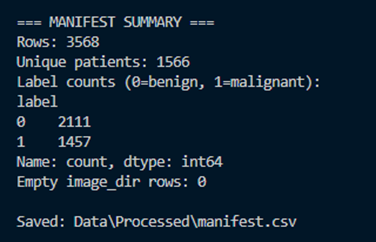
\includegraphics[width=0.95\linewidth]{figures/featureprototype/terminal1.png}
  \caption{Terminal output from the preprocessing/manifest step.}
  \label{fig:terminal1}
\end{figure}

To prevent data leakage, the dataset is split at the patient level rather than the image level, something that I explored in the literature review and the design section of the report. This is a critical consideration in medical imaging tasks, where multiple images from the same patient can otherwise appear in both training and evaluation sets, leading to inflated performance estimates. The splitting logic is implemented in \texttt{split\_data.py} using scikit-learn’s GroupShuffleSplit, with the patient identifier used as the grouping variable. The data is divided into training, validation, and test subsets according to proportions defined in the configuration file, ensuring that no patient appears in more than one split.

\texttt{Split\_data.py}, how GroupShuffleSplit is used with \texttt{patient\_id} as the grouping variable:

\lstinputlisting[
  language=Python,
  firstline=6,
  lastline=47,
    caption={how GroupShuffleSplit is used with \texttt{patient\_id} as the grouping variable in \texttt{split\_data.py}},
    label={lst:split_data}
]{../SRC/split_data.py}

Image loading and preprocessing are handled by a custom PyTorch Dataset class implemented in dataset.py. Because CBIS-DDSM images are stored as DICOM files, standard image loading utilities wouldn’t be sufficient. Instead, I used the pydicom library to read pixel data directly from the DICOM files. For this baseline implementation, a single representative DICOM image is loaded from each image series directory. Pixel intensities are normalised to the range [0, 1] to stabilise training, and images are resized to a fixed resolution compatible with the CNN architecture. Other data augmentation, including random horizontal flips and small rotations, is applied during training to improve generalisation.

The architecture used in this project is ResNet, selected in line with the design decisions outlined in Chapter 3. Transfer learning is employed by initialising the network with ImageNet pretrained weights. Given that mammography images are grayscale, the first convolutional layer of the network is adapted to accept a single channel input by averaging the RGB weights. The final fully connected layer is replaced with a single output neuron, producing a single logit suitable for binary classification using a sigmoid based loss function.

Code snippet for \texttt{model.py}:

\lstinputlisting[
  language=Python,
  firstline=5,
  lastline=29,
    caption={Model definition and transfer learning setup in \texttt{model.py}},
    label={lst:model}
]{../SRC/model.py}

Training logic is implemented in \texttt{train.py}. This script loads the previously generated manifest, applies the patient-level splitting procedure, and constructs PyTorch data loaders for the training and validation sets. Model performance on the validation set is monitored at the end of each epoch, and the best performing model checkpoint is saved automatically. This ensures that evaluation is conducted on the most generalisable model rather than the final training state, which may be overfitted.

Training loop from \texttt{train.py}:

\lstinputlisting[
  language=Python,
  firstline=170,
  lastline=219,
    caption={Training loop in \texttt{train.py}},
    label={lst:train_loop}
]{../SRC/train.py}

The model was trained for 10 epochs using ResNet initialised with ImageNet pretrained weights. Validation performance was monitored at the end of each epoch, and the model checkpoint achieving the lowest validation loss was saved automatically.

Across training, both training loss and validation loss decreased steadily, indicating effective learning without immediate signs of severe overfitting. Validation accuracy improved from approximately 63\% after the first epoch to just over 70\% by the final epoch.

\begin{figure}[H]
  \centering
  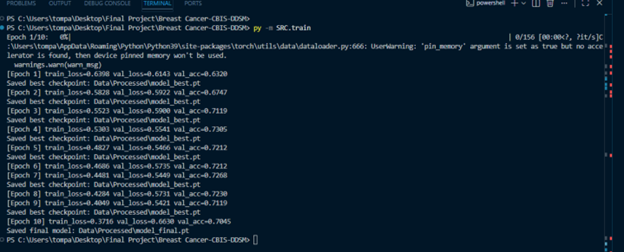
\includegraphics[width=0.95\linewidth]{figures/featureprototype/terminal2.png}
  \caption{Terminal output training over 10 epochs.}
  \label{fig:terminal2}
\end{figure}

Evaluation is performed using a separate script, eval.py, which loads the saved test split and the best model checkpoint. The model produces probability estimates for each test sample, which are then used to compute relevant evaluation metrics. These metrics include the area under the receiver operating characteristic curve (AUC), precision, recall (sensitivity), specificity, F1 score, and confusion matrix values. The results are printed to the terminal for inspection and saved to a structured JSON file to support reproducibility and reporting. Whilst this is presentable, I am considering an implementation which better displays the result, possibly with some kind of GUI. However, this would be a late project extension if that was a direction in which I wished to take the project once fully operational.

Final evaluation was conducted on a held-out test set containing data from patients unseen during training and validation. The best performing model checkpoint was loaded and used to generate probabilistic predictions for each test sample. At a decision threshold of 0.5, the model achieved the following results:

\begin{figure}[H]
  \centering
    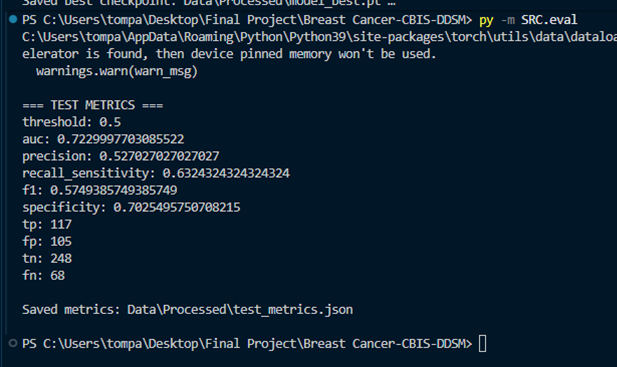
\includegraphics[width=0.95\linewidth]{figures/featureprototype/terminal3.png}
    \caption{Terminal output from the evaluation step.}
    \label{fig:terminal3}
\end{figure}

The confusion matrix at this threshold contained 117 true positives, 248 true negatives, 105 false positives, and 68 false negatives. These results indicate that the model demonstrates reasonable discriminative ability, with particular strength in sensitivity relative to random or majority class baselines.

While false positives remain relatively high, this does give a solid foundation to build upon as the project moves forward.

The prototype demonstrates that the proposed system design is technically feasible and can be implemented in a structured, reproducible manner. The modular architecture allows individual components to be modified or extended independently, such as replacing the backbone network, incorporating class weighting to address imbalance, or extending the dataset loader to use multiple DICOM images per study.

\section{Baseline Results}

This section reports the baseline performance of the trained classifier evaluated on a held-out test set
containing data from patients unseen during training and validation. All results presented here therefore
reflect patient-level generalisation performance rather than image-level memorisation.

Given the clinical context of breast cancer screening, a conservative operating point was selected.
Rather than using the default decision threshold of 0.5, the classification threshold was adjusted to
achieve approximately 90\% specificity. This reflects a screening-oriented deployment scenario in which
limiting false positive cases is important to reduce unnecessary follow-up investigations and patient
anxiety, while still retaining reasonable sensitivity. The resulting threshold was approximately
$\tau \approx 0.620$.

Table~\ref{tab:baseline_metrics} summarises the primary performance metrics achieved at this
specificity-constrained operating point. In addition to aggregate metrics such as ROC--AUC and average
precision, clinically interpretable measures including sensitivity, specificity, and the confusion matrix
counts are reported.

\begin{table}[H]
\centering
\begin{tabular}{lr}
\toprule
Metric & Value \\
\midrule
Decision threshold (spec $\approx$ 0.90) & 0.6205 \\
ROC--AUC & 0.7454 \\
Average Precision (AP) & 0.5996 \\
Precision & 0.6413 \\
Recall / Sensitivity & 0.3189 \\
Specificity & 0.9065 \\
F1-score & 0.4260 \\
\midrule
TP / FP / TN / FN & 59 / 33 / 320 / 126 \\
\bottomrule
\end{tabular}
\caption{Baseline test performance at the specificity-constrained operating point.}
\label{tab:baseline_metrics}
\end{table}

At this operating point, the model achieves a specificity of approximately 90.7\%, indicating that the
majority of non-cancer cases are correctly classified. However, this comes at the cost of reduced
sensitivity, with only 31.9\% of malignant cases correctly identified. This trade-off highlights the
difficulty of achieving both high sensitivity and high specificity in highly imbalanced screening datasets.

The confusion matrix for this operating point is shown in Figure~\ref{fig:cm_baseline}. The relatively low
number of false positives compared to true negatives reflects the specificity constraint, while the
presence of a substantial number of false negatives underscores the limitations of the baseline model in
detecting all cancer-positive cases.

\begin{figure}[H]
  \centering
  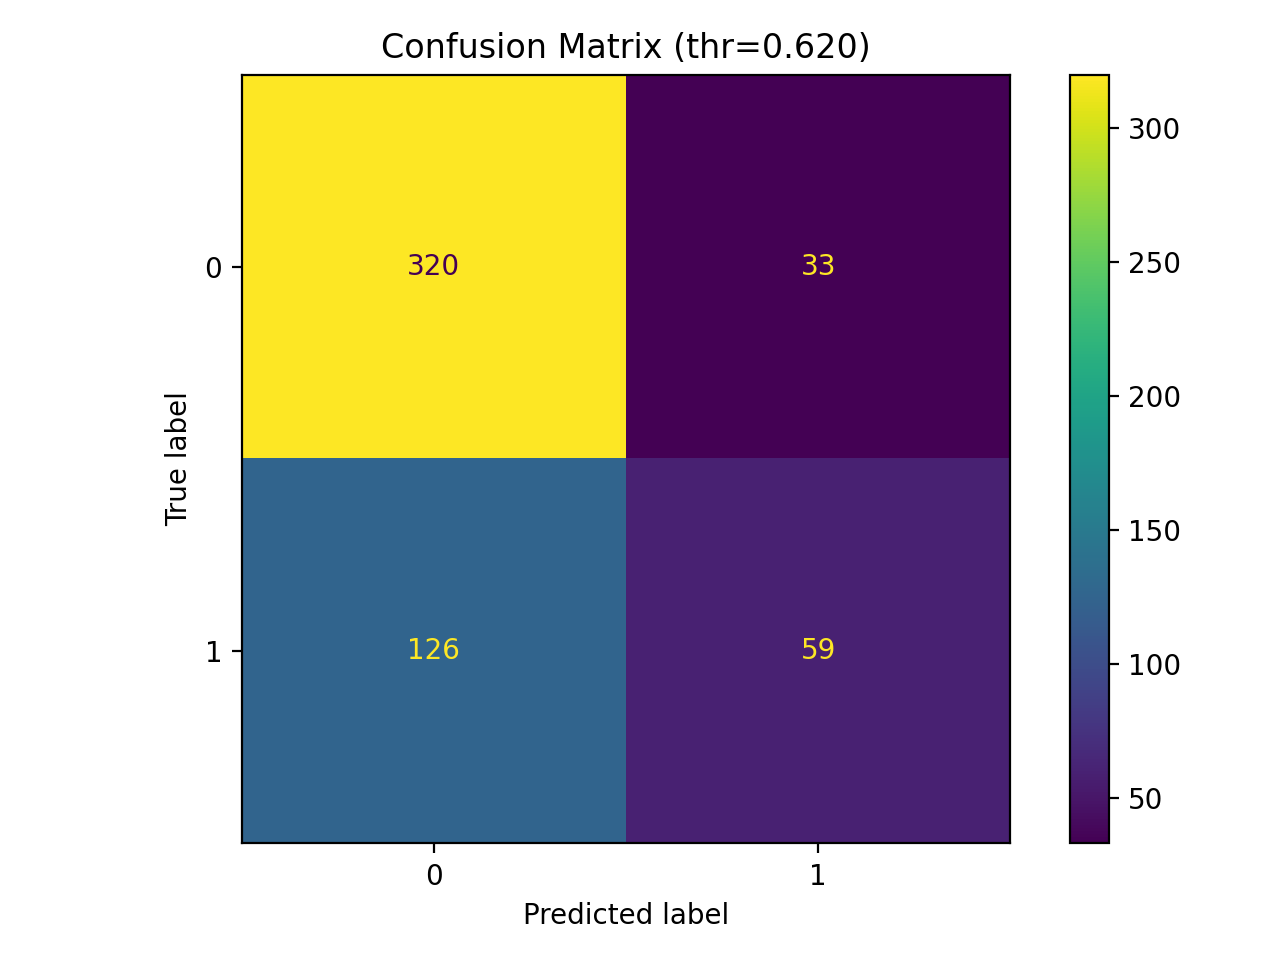
\includegraphics[width=0.75\linewidth]{figures/baseline/confusion_matrix_thr_spec0.90.png}
  \caption{Baseline confusion matrix at the specificity-constrained threshold (thr $\approx 0.620$).}
  \label{fig:cm_baseline}
\end{figure}

Figure~\ref{fig:roc_baseline} presents the receiver operating characteristic (ROC) curve for the baseline
model. The ROC--AUC of approximately 0.745 indicates that the classifier demonstrates reasonable
discriminative ability, performing substantially better than random chance. However, AUC alone does not
fully capture clinical usefulness in imbalanced datasets, motivating the inclusion of additional evaluation
metrics.

\begin{figure}[H]
  \centering
  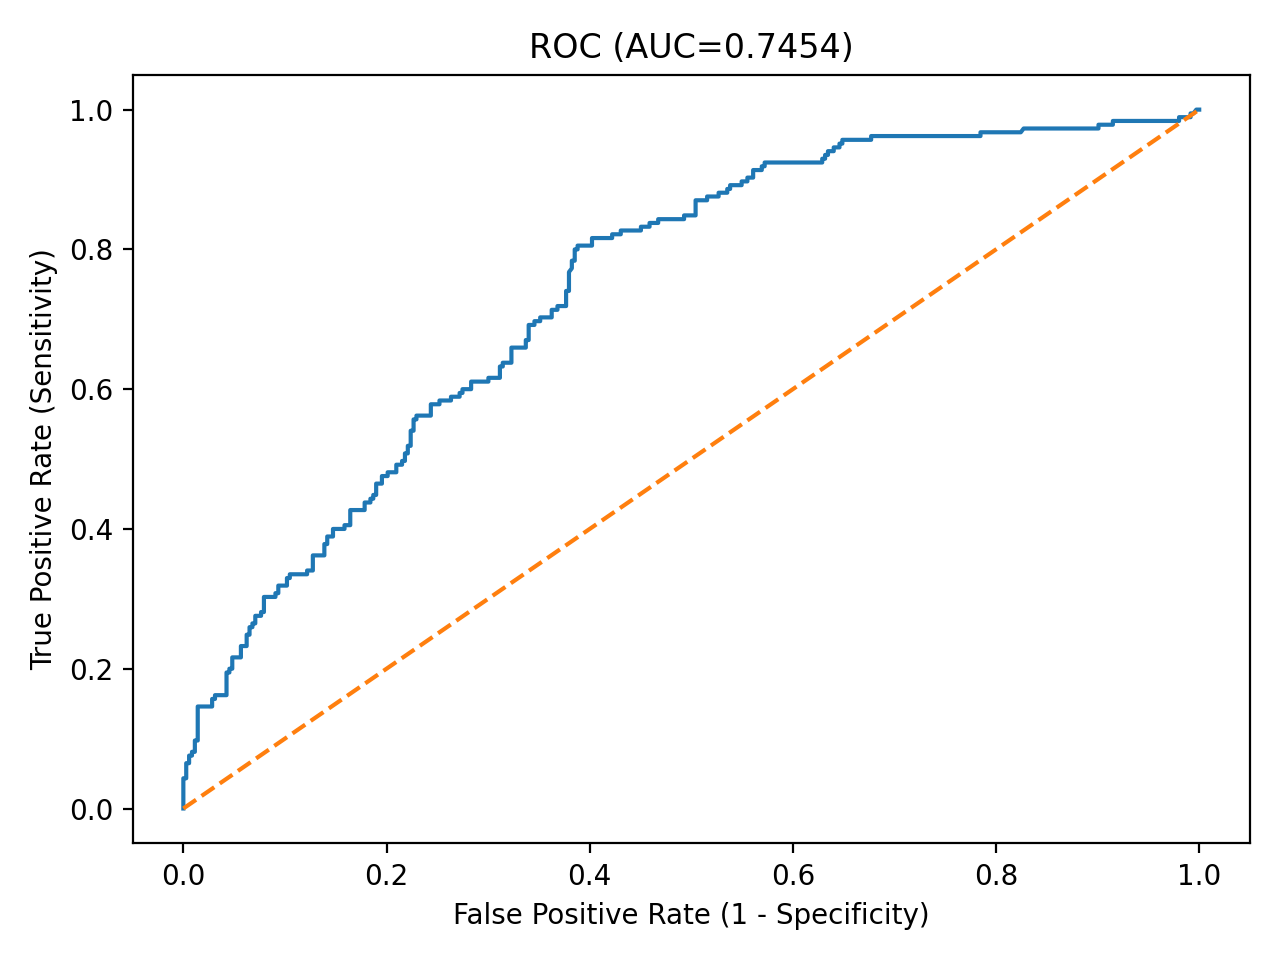
\includegraphics[width=0.75\linewidth]{figures/baseline/roc_curve.png}
  \caption{ROC curve for the baseline model (AUC $\approx 0.745$).}
  \label{fig:roc_baseline}
\end{figure}

The precision--recall (PR) curve is shown in Figure~\ref{fig:pr_baseline}. The average precision of
approximately 0.60 reflects the challenge of maintaining high precision while increasing recall in a
screening context where malignant cases are relatively rare. The PR curve provides a more informative
view of performance than ROC curves under class imbalance, particularly with respect to false positive
and false negative trade-offs.

\begin{figure}[H]
  \centering
  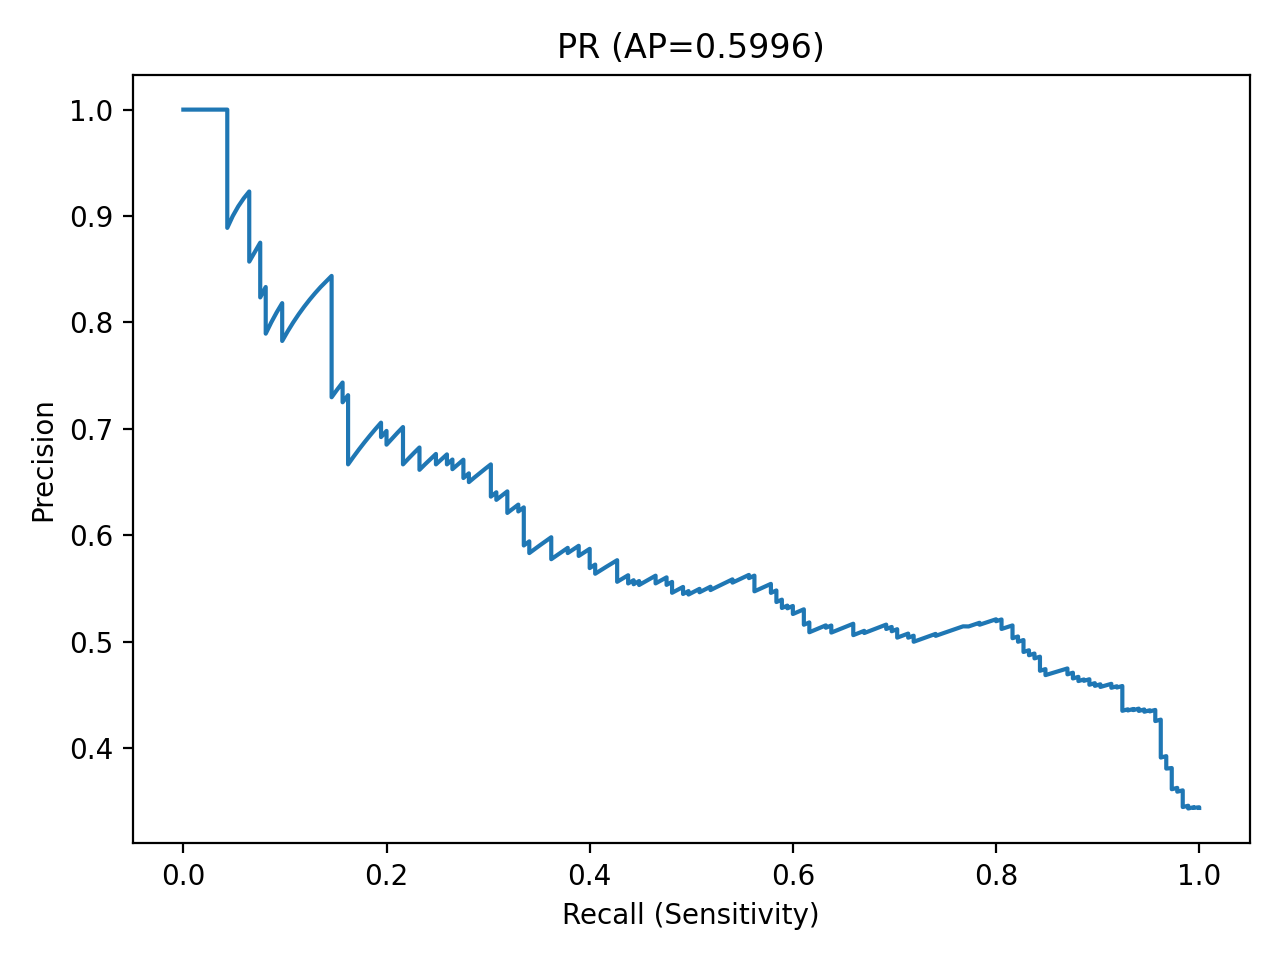
\includegraphics[width=0.75\linewidth]{figures/baseline/pr_curve.png}
  \caption{Precision--Recall curve for the baseline model (AP $\approx 0.600$).}
  \label{fig:pr_baseline}
\end{figure}

Finally, model calibration is assessed using the reliability diagram shown in
Figure~\ref{fig:cal_baseline}. While the predicted probabilities broadly follow the ideal diagonal trend,
deviations are visible across several bins, suggesting that the model is not perfectly calibrated. This
indicates that predicted confidence scores may not always correspond directly to true outcome
probabilities, which is an important consideration for human-in-the-loop deployment scenarios.

\begin{figure}[H]
  \centering
  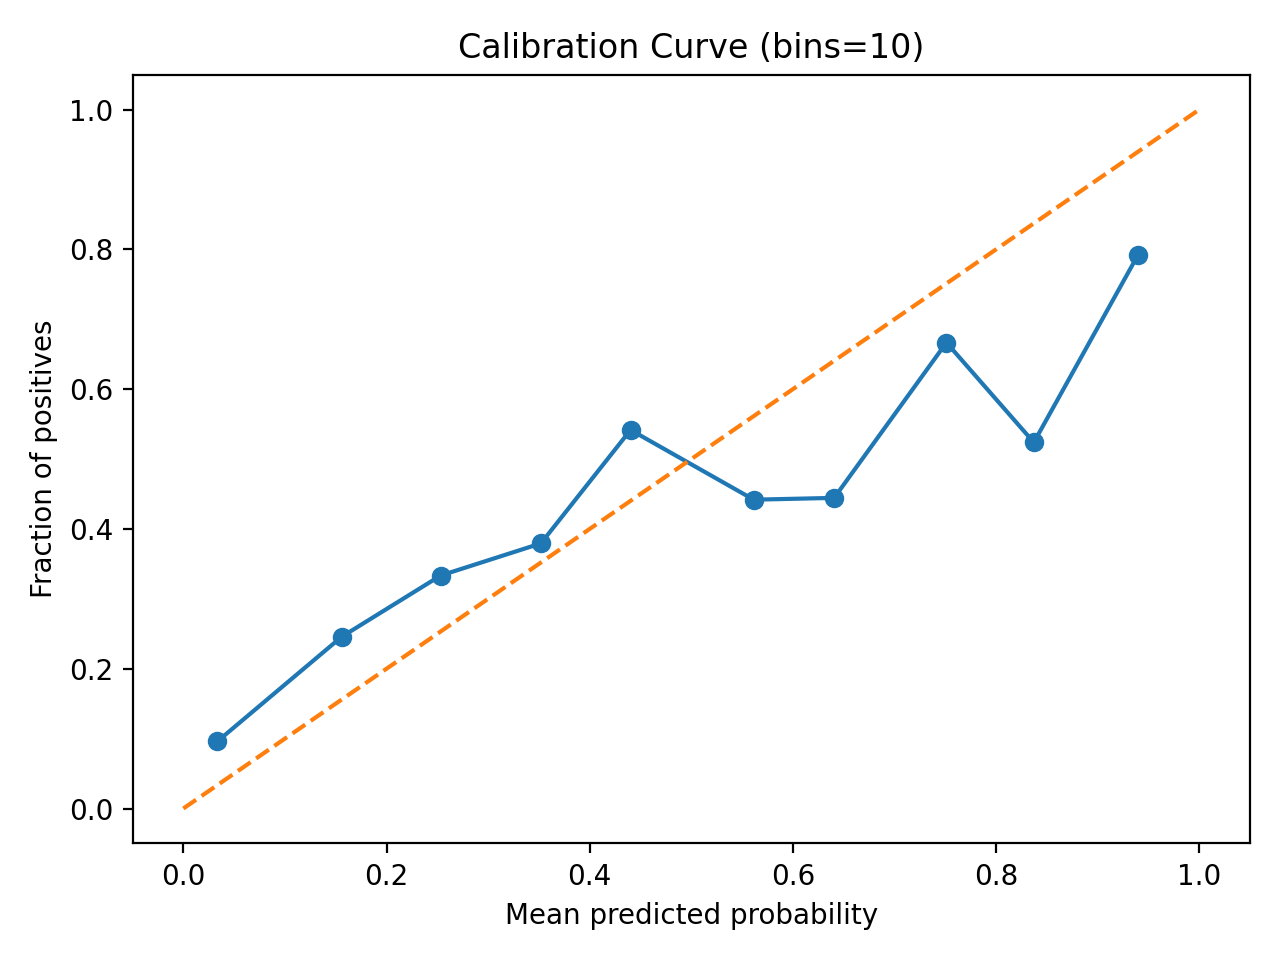
\includegraphics[width=0.75\linewidth]{figures/baseline/calibration_curve.png}
  \caption{Calibration curve for the baseline model (10 bins).}
  \label{fig:cal_baseline}
\end{figure}

Overall, these baseline results demonstrate that the proposed pipeline is capable of learning meaningful
discriminative features from mammography images, while also highlighting clear limitations in sensitivity
and calibration. These results establish a reference point against which subsequent architectural,
training, and evaluation refinements can be compared.


\section{Methodology}

\begin{table}[ht]
\centering
\caption{Effect of \texttt{pos\_weight} at an operating point targeting specificity $\approx 0.90$ (seed=42).}
\label{tab:pos_weight_sweep}
\begin{tabular}{rcccccccc}
\hline
pos\_weight & ROC AUC & AP & Spec & Sens & Prec & F1 & TP/FP/TN/FN & Thr@Spec$\approx$0.90 \\
\hline
1 & 0.7294 & 0.5758 & 0.9008 & 0.3189 & 0.6277 & 0.423 & 59/35/318/126 & 0.7979 \\
2 & 0.7373 & 0.6085 & 0.9008 & 0.3405 & 0.6429 & 0.445 & 63/35/318/122 & 0.8982 \\
3 & 0.7454 & 0.5996 & 0.9065 & 0.3189 & 0.6413 & 0.426 & 59/33/320/126 & 0.6205 \\
5 & 0.7551 & 0.5925 & 0.9093 & 0.3135 & 0.6444 & 0.422 & 58/32/321/127 & 0.9276 \\
\hline
\end{tabular}
\end{table}


We select \texttt{pos\_weight}=2 for subsequent runs because it yields the highest sensitivity at specificity $\approx 0.90$.

\begin{table}[ht]
\centering
\caption{Augmentation ablation at fixed operating point (target specificity $\approx 0.90$), with \texttt{pos\_weight}=2 (seed=42).}
\label{tab:augmentation_ablation}
\begin{tabular}{lcccccccc}
\hline
Setting & ROC AUC & AP & Spec & Sens@Spec$\approx$0.90 & Thr@Spec$\approx$0.90 & TP/FP/TN/FN \\
\hline
Augmentation ON  & 0.7294 & 0.5758 & 0.9008 & 0.3189 & 0.7979 & 59/35/318/126 \\
Augmentation OFF & 0.7524 & 0.6181 & 0.9008 & 0.3730 & 0.9012 & 69/35/318/116 \\
\hline
\end{tabular}
\end{table}



Disabling augmentation improved sensitivity at fixed specificity ($\approx 0.90$), so augmentation was disabled for subsequent experiments.

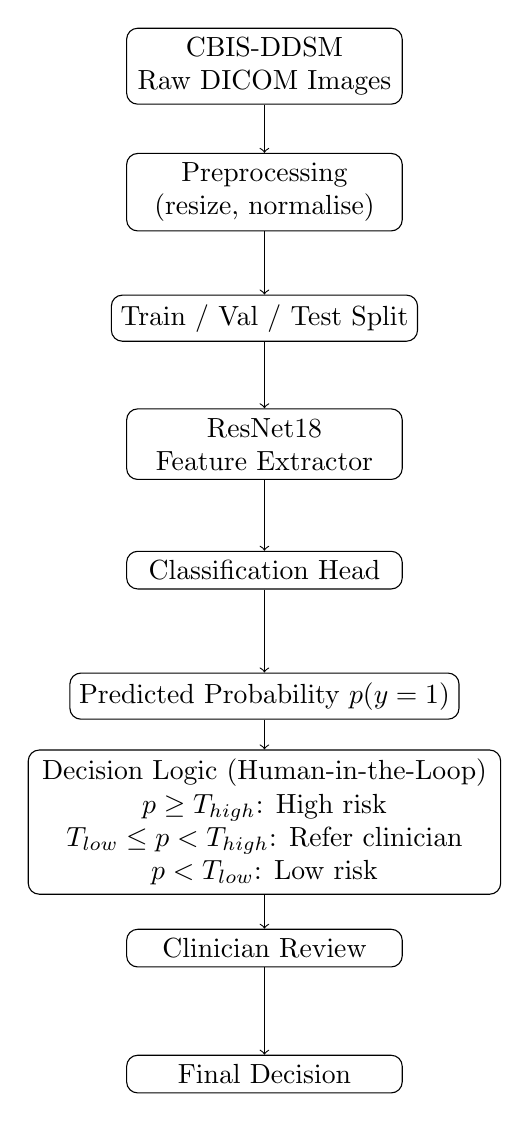
\begin{tikzpicture}[
    node distance=1.6cm,
    every node/.style={draw, rectangle, rounded corners, align=center, minimum width=3.5cm}
]

\node (data) {CBIS-DDSM\\Raw DICOM Images};
\node (prep) [below of=data] {Preprocessing\\(resize, normalise)};
\node (split) [below of=prep] {Train / Val / Test Split};
\node (cnn) [below of=split] {ResNet18\\Feature Extractor};
\node (head) [below of=cnn] {Classification Head};
\node (prob) [below of=head] {Predicted Probability $p(y=1)$};

\node (decision) [below of=prob, minimum width=6cm] {
Decision Logic (Human-in-the-Loop)\\
$p \geq T_{high}$: High risk\\
$T_{low} \leq p < T_{high}$: Refer clinician\\
$p < T_{low}$: Low risk
};

\node (human) [below of=decision] {Clinician Review};
\node (outcome) [below of=human] {Final Decision};

\draw[->] (data) -- (prep);
\draw[->] (prep) -- (split);
\draw[->] (split) -- (cnn);
\draw[->] (cnn) -- (head);
\draw[->] (head) -- (prob);
\draw[->] (prob) -- (decision);
\draw[->] (decision) -- (human);
\draw[->] (human) -- (outcome);

\end{tikzpicture}


\nocite{*}
\input{sections/bibliography}


\end{document}
